\documentclass{article}

\usepackage{amsmath}
\usepackage{amssymb}
\usepackage{amsthm}
\usepackage{array}
\usepackage[T1]{fontenc}
\usepackage{geometry}
\usepackage{graphicx}
\usepackage{semantic}

\theoremstyle{definition}
\newtheorem{theorem}{Theorem}
\newtheorem{corollary}{Corollary}
\newtheorem{lemma}{Lemma}
\newtheorem{definition}{Definition}

\newcommand{\at}{\ensuremath{{\scriptstyle{@}}}}
\newcommand{\pc}{\ensuremath{{\mathit{pc}}}}

\newcommand{\CoqSymbol}
{\raisebox{-.2ex}{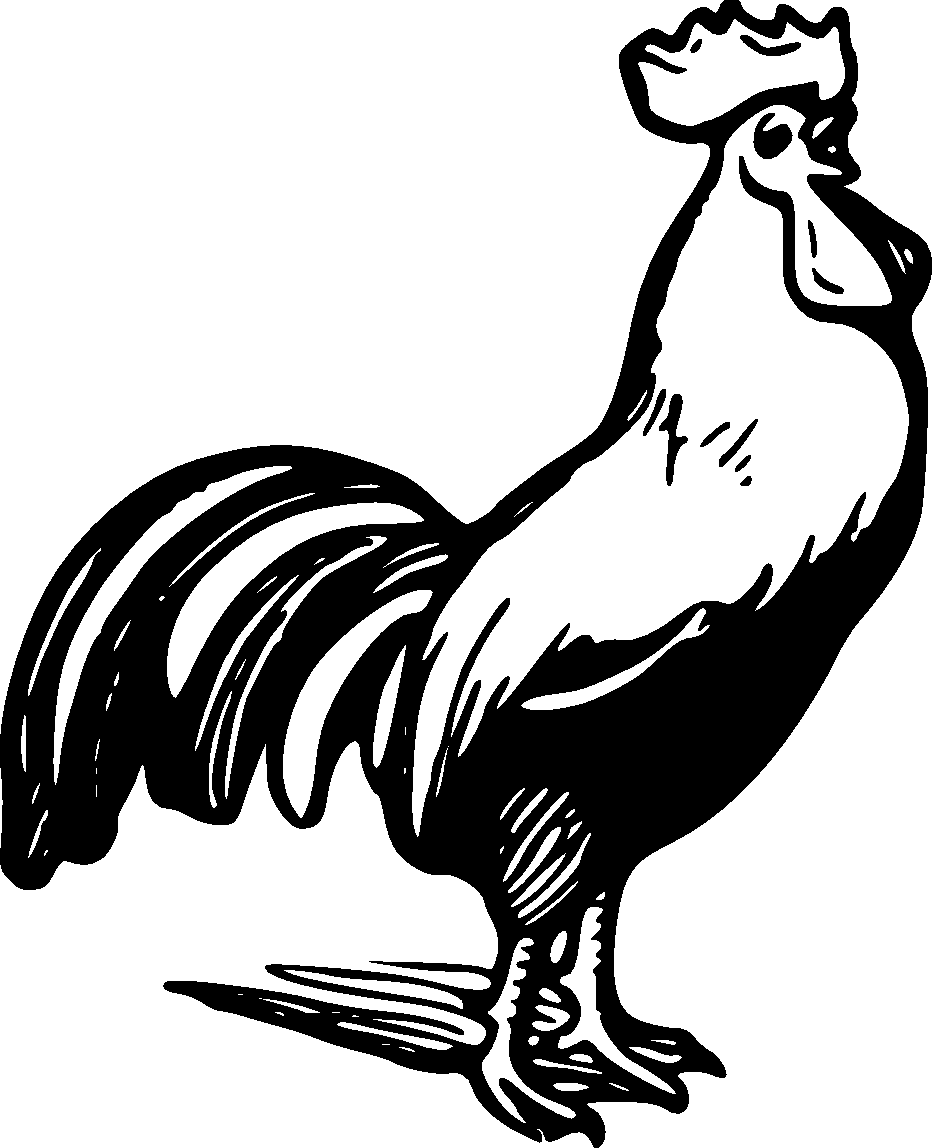
\includegraphics[height=0.9em]{coq.pdf}}\,}
\newcommand{\Coqed}{\hfill\CoqSymbol}

\renewcommand*{\descriptionlabel}[1]{\hspace\labelsep\normalfont #1}

\begin{document}

\begin{flushright}
  \today
\end{flushright}

\begin{figure}[ht]
  \centering
  \[
  \mathcal{L} = \{ \bot, \top \}
  \qquad
  \bot \sqsubseteq \top
  \qquad
  L^{\mathit{def}} = \bot
  \qquad
  \mathcal{A} = \mathbf{1}
  \]
  \begin{array}[t]{lcl}
    b & ::= &
    \mathit{tt}\;\; |\;\;
    \mathit{ff}
    \\[0.3ex]
    c & :: = &
    b\;\; |\;\;
    n
    \\[0.3ex]
    e & ::= &
    c\;\; |\;\;
    x\;\; |\;\;
    \lambda{x}.\, e\;\; |\;\;
    e\ e\;\; |\;\;
    \mathsf{declassify}\ e\ e
    \\[0.3ex]
    v & ::= &
    c\;\; |\;\;
    \langle{\rho, \lambda{x}.\, e\rangle}
    \\[0.3ex]
    a & ::= &
    v \at L
    \\[0.3ex]
    \rho & ::= &
    \bullet\;\; |\;\;
    \rho, x = a
  \end{array}
  \caption{Syntax of $\lambda_{\mathbf{2}}$.}
  \label{fig:syntax}
\end{figure}

\begin{figure}[ht]
  \centering
  \begin{gather*}
    \inference{}{
      \pc, \rho |- c \Downarrow^{k} c \at \pc
    }[\textsc{E-Const}]
    \qquad
    \inference{
      {\begin{array}{l}
          \rho(x) = v \at L
        \end{array}}
    }{
      \pc, \rho |- x \Downarrow^{k} v \at (\pc \sqcup L)
    }[\textsc{E-Var}]
    \\[3ex]
    \inference{}{
      \pc, \rho |- (\lambda{x}.\, e) \Downarrow^{k}
      \langle{\rho, \lambda{x}.\, e\rangle} \at \pc
    }[\textsc{E-Abs}]
    \qquad
    \inference{
      {\begin{array}{l}
          \pc, \rho |- e_1 \Downarrow^{k}
          \langle{\rho_1, \lambda{x}.\, e\rangle} \at L_1
          \\
          \pc, \rho |- e_2 \Downarrow^{k} a_2
          \\
          L_1, (\rho_1, x = a_2) |- e \Downarrow^{k} a_3
        \end{array}}
    }{
      \pc, \rho |- (e_1\ e_2) \Downarrow^{k+1} a_3
    }[\textsc{E-App}]
    \\[3ex]
    \inference{
      {\begin{array}{l}
          \pc, \rho |- (e_1\ e_2) \Downarrow^{k} v \at \bot
        \end{array}}
    }{
      \pc, \rho |- (\mathsf{declassify}\ e_1\ e_2) \Downarrow^{k+1}
      v \at \bot
    }[\textsc{E-Decl1}]
    \\[3ex]
    \inference{
      {\begin{array}{l}
          \pc, \rho |- e_1 \Downarrow^{k}
          \langle{\rho_1, \lambda{x}.\, e\rangle} \at L_1
          \\
          \pc, \rho |- e_2 \Downarrow^{k} a_2
          \\
          L_1, (\rho_1, x = a_2) |- e \Downarrow^{k} v_3 \at \top
          \\
          \forall{\rho_1', a_2' \text{ s.t. }
            (\rho_1, x = a_2) \approx^{L}_{P} (\rho_1', x = a_2')}.
          \\\quad
          L_1, (\rho_1', x = a_2') |- e \Downarrow^{k} v_3' \at \top =>
          v_3 \approx^{L}_{P} v_3'
        \end{array}}
    }{
      \pc, \rho |- (\mathsf{declassify}\ e_1\ e_2) \Downarrow^{k+1}
      v_3 \at \bot
    }[\textsc{E-Decl2}]
  \end{gather*}
  \caption{Semantics of $\lambda_{\mathbf{2}}$.}
  \label{fig:semantics}
\end{figure}

\pagebreak

\begin{definition}
  The $\approx^{L}_{P}$ relation expresses the \emph{indistinguishability} of
  atoms for observers at label $L$ and with respect to some reflexive relation
  $P$, where $v_1 \at L_1 \approx^{L}_{P} v_2 \at L_2$ iff either
  \begin{itemize}
  \item
    $L = \bot$ and
    $L_1 = L_2 = \top$ and either
    \begin{itemize}
    \item
      $v_1 = n_1$ and
      $v_2 = n_2$ and
      $P(v_1, v_2)$, or
    \item
      $v_1 = \langle{\rho_1, \lambda{x_1}.\, e_1\rangle}$ and
      $v_2 = \langle{\rho_2, \lambda{x_2}.\, e_2\rangle}$ and
      $v_1 \approx^{L}_{P} v_2$, or
    \item
      $v_1 = c_1$ and $v_2 = \langle{\rho_2,\lambda{x_2}.\, e_2\rangle}$, or
    \item
      $v_1 = \langle{\rho_1, \lambda{x_1}.\, e_1\rangle}$ and $v_2 = c_2$; or
    \end{itemize}
  \item $L = \bot$ and
    $L_1 = L_2 = \bot$ and $v_1 \approx^{L}_{P} v_2$; or
  \item $L = \top$ and $L_1 = L_2$ and $v_1 \approx^{L}_{P} v_2$.
  \end{itemize}
  The definition for atoms is mutually recursive with that for values and
  environments:
  \begin{itemize}
  \item $c_1 \approx^{L}_{P} c_2$ iff $c_1 = c_2$.
  \item
    $\langle{\rho_1, \lambda{x_1}.\, e_1\rangle} \approx^{L}_{P}
    \langle{\rho_2, \lambda{x_2}.\, e_2\rangle}$ iff
    $\rho_1 \approx^{L}_{P} \rho_2$ and
    $\lambda{x_1}.\, e_1 \equiv \lambda{x_2}.\, e_2$.
  \item $\rho_1 \approx^{L}_{P} \rho_2$ iff
    $\mathrm{dom}\; \rho_1 = \mathrm{dom}\; \rho_2$ and
    $\rho_1(x) \approx^{L}_{P} \rho_2(x)$ for every
    $x \in \mathrm{dom}\; \rho_1$.
  \end{itemize}
  We write $\approx^{L}$ when $P$ is the everywhere-true or everywhere-false
  predicate.
  \label{def:lp-equiv}
\end{definition}

\begin{lemma}
  $\approx^{L}_{P}$ implies $\approx^{L}$.
  \begin{enumerate}
  \item If $a_1 \approx^{L}_{P} a_2$, then $a_1 \approx^{L} a_2$.
  \item If $v_1 \approx^{L}_{P} v_2$, then $v_1 \approx^{L} v_2$.
  \item If $\rho_1 \approx^{L}_{P} \rho_2$, then $\rho_1 \approx^{L} \rho_2$.
  \Coqed
  \end{enumerate}
  \label{lem:lp-equiv-l-equiv}
\end{lemma}

\begin{lemma}
 If $v_1 \at L_1 \approx^{L}_{P} v_2 \at L_2$, then $L_1 = L_2$.
 \Coqed
 \label{lem:lp-equiv-lab-inv}
\end{lemma}

\begin{lemma}
  If $v_1 \at \bot \approx^{L}_{P} v_2 \at \bot$, then
  $v_1 \at \top \approx^{L}_{P} v_2 \at \top$.
  \Coqed
  \label{lem:lp-equiv-raise}
\end{lemma}

\begin{theorem}
  If $\pc, \rho |- e \Downarrow^{k} a$ and
  $\pc, \rho' |- e \Downarrow^{k} a'$
  and $\rho \approx^{L}_{P} \rho'$, then
  $a \approx^{L}_{P} a'$.
  \Coqed
  \label{them:non-interference}
\end{theorem}

\end{document}
